% !TEX root = main.tex
\section{Dettagli implementativi}
L'applicazione adotta un'architettura local-first cioè tutta l'elaborazione dei dati e le funzioni principali dell'app come il calcolo dei pesi e l'inferenza del modello avvengono sul dispositivo, l'unica interazione con la rete è il download periodico dei prezzi. I motivi dietro questa scelta sono:
\begin{itemize}
    \item \textbf{Privacy e autonomia}: i portafogli dell'utente, le allocazioni e i risultati non lasciano mai il dispositivo.
    \item \textbf{Funzionamento offline}: dopo la prima sincronizzazione l'app resta completamente utilizzabile anche senza connessione in quanto tutti i dati utili al suo funzionamento risiedono in un database locale.
    \item \textbf{Costo nullo di infrastruttura}: non essendoci un backend da mantenere, l'aggiornamento dei dati è delegato a un servizio di automazione gratuito, evitando qualsiasi hosting dedicato.

\end{itemize}
In sostanza c'è un separazione tra due sottosistemi: una pipeline di produzione del dato e un sottosistema di consumo e persistenza.
\subsubsection{Sorgente e struttura del dato}
\label{sec:sorgente e struttura del dato}
I dati di mercato sono ottenuti da Yahoo Finance tramite la libreria \lstinline{yfinance}. 
L'universo scaricato è l'intero indice S\&P500: l'elenco dei ticker è estratto a runtime dalla pagina di Wikipedia dell'indice, in modo da garantire l'aggiornamento automatico della composizione qualora dovesse cambiare nel tempo, nel caso in cui Wikipedia non dovesse essere raggiungibile viene usata una lista statica dei titoli nell'S\&P500.
Per ogni titolo viene acquisita una storia di tre anni di dati giornalieri, con la modalità \lstinline{auto_adjust = True} come per il modello. Le feature che vengono conservate sono le quattro feature di mercato utilizzate dal modello cioè high, low, close e VIX, l'open non viene memorizzata in quanto non viene utilizzata da alcun metodo. 
Il download avviene un ticker alla volta e non in blocco, in questo modo vengono prodotte serie a indice singolo più semplici e robuste da elaborare, e permette di isolare i fallimenti.
\subsubsection{Pipeline di aggiornamento automatico}
L'aggiornamento è affidato a un workflow di GitHub Actions, l'esecuzione avviene alle 22:00 UTC nei giorni feriali, ovvero dopo la chiusura del mercato statunitense. Il workflow:
\begin{enumerate}
    \item predispone un ambiente Python ed installa le dipendenze;
    \item esegue lo script di download, che produce il dataset;
    \item effettua il commit del dataset aggiornato nel repository.
\end{enumerate}
Il repository Git assume il ruolo di archivio versionato dei dati e punto di distribuzione verso i client.
Con tutti gli storici dei 503 titoli però esso raggiunge dimensioni di circa 33MB che è una dimensione molto grande per essere scaricata sui dispositivi mobili.
\subsection{Datasets}
\label{sec:datasets}
Il Dataset è in formato JSON, con due collezzioni principali: \lstinline{prices} e \lstinline{market}. 
Per questo motivo viene applicata una conversione gzip al momento della generazione del dataset: lo script genera accanto al JSON una versione compressa che pesa circa 5,4MB. 
La versione gzip è quella effettivamente usata, lato client la decompressione avviene attraverso la libreria \lstinline{fflate}, in javascript puro.

\subsubsection{Database locale}
\label{subsec:database locale}
Sul dispositivo i dati vengono racchiusi in un database SQLite, interrogato tramite l'ORM tipizzato Drizzle. 
Lo schema è minimale e normalizzato, ed è diviso nelle seguenti tabelle:
\begin{figure}[H]
  \centering
  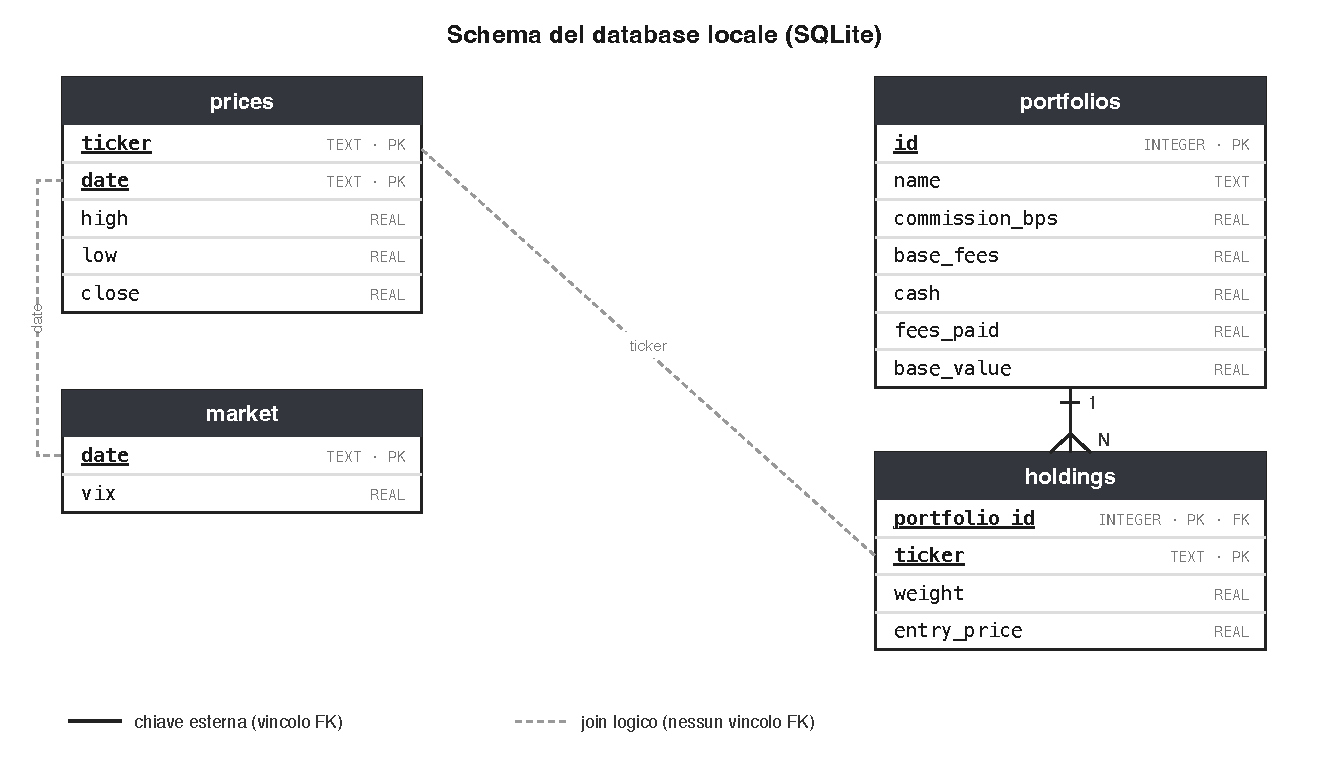
\includegraphics[width=0.95\textwidth]{er_diagram.pdf}
  Le chiavi primarie composte
  \texttt{(ticker,\,date)} e \texttt{(portfolio\_id,\,ticker)}
  impediscono che ci siano dati duplicati.
  L'unica relazione con vincolo di integrità
  referenziale è \texttt{holdings.portfolio\_id} $\rightarrow$
  \texttt{portfolios.id}.
  \label{fig:er-schema}
\end{figure}

SQLite su dispositivi mobili ha un limite di variabili che può gestire con un'unica query.
Per risolvere questo problema i dati vengono divisi in array da al massimo 500 elementi ciascuno.
I dati vengono quindi inseriti un blocco alla volta all'interno del database in modo da evitare errori.

L'evoluzione dello schema è gestita in maniera standard tramite migrazioni versionate, ovvero degli script sequenziali che modificano la struttura dei dati per adattarla ai requisiti del software.
Queste migrazioni vengono generate in fase di sviluppo e applicate automaticamente all'avvio, prima di ogni accesso ai dati. 
Un registro interno al database memorizza lo storico degli aggiornamenti assicurando che ogni migrazione venga applicata una sola volta.
In questo modo se il database è già allineato all'ultima versione l'aggiornamento si conclude senza eseguire nessuna istruzione.

\subsubsection{Sincronizzazione lato applicazione}

All'avvio, dopo le migrazioni, l'app esegue la procedura di sincronizzazione, che svolge tre operazioni fondamentali.
\begin{itemize}
  \item \textbf{Limitazione di frequenza}: una tabella di servizio conserva la data dell'ultima sincronizzazione e se coincide con quella odierna impedisce che vengano fatte altre sincronizzazioni.
  \item \textbf{Inserimento idempotente}: come descritto nella sezione precedente i dati vengono inseriti a blocchi.
  In caso di conflitto sulle chiavi primarie la riga esistente viene aggiornata con i valori
  piu' recenti. In questo modo si evitano duplicazioni di dati.
  \item \textbf{Finestra temporale mobile}: ad ogni sincronizzazione vengono scaricati gli ultimi tre anni di storico. 
  Si scaricano gli interi tre anni perché \lstinline{yfinance} con \lstinline{auto_adjust=True} aggiorna i prezzi compresi quelli passati ad ogni split e dividendo, quindi vanno sovrascritti.
  Per tenere lo spazio occupato costante vengono eliminati di volta in volta tutti i record corrispondenti a date precedenti alla prima data nel dataset scaricato.
\end{itemize}

\subsubsection{Inizializzazione e primo avvio}

L'applicazione include un seed iniziale di dati impacchettati nel bundle per garantire l'usabilità anche in assenza di rete alla prima apertura. 
Al primissimo avvio, se la tabella dei prezzi è vuota, il seed la popola. 
Successivamente la sincronizzazione allinea il contenuto alla versione più recente. 
Le tre fasi di sincronizzazione avvengono con frequenze diverse: le migrazioni sono verificate a ogni avvio ma applicate una sola volta, il seed viene eseguito solo a database vuoto, la sincronizzazione al più una volta al giorno.

\subsubsection{Limiti}
Si espongono in questa sezione limiti progettuali dell'app.
I dati vengono scaricati solo una volta al giorno e sono i prezzi a chiusura del mercato, non ci sono quindi dati in tempo reale.
L'API di \lstinline{yfinance} si appoggia a end-point non ufficiale di Yahho Finance, il servizio può cambiare senza preavviso e richiederebbe manutenzione dello script.
La distribuzione via repository nn è pensata come canale ad alto volume, funziona bene per essere usata da pochi utenti ma se diventano migliaia non reggerebbe la concorrenza.

\subsection{Esecuzione del modello on-device}
\label{subsec:inferenza-onnx}

Il modello discusso nella sezione~\ref{sec:modello} viene addestrato in Python ed esportato in formato ONNX (Open Neural Network Exchange).
ONNX è uno standard e serve a disaccoppiare il framework di addestramento dal motore di esecuzione.
In questo modo è possibile far girare il modello in un ambiente React Native direttamente sul dispositivo.

L'inferenza quindi avviene in locale utilizzando la libreria \lstinline{onnxruntime-react-native} che esegue il modello sulla CPU del dispositivo.
Non è previsto alcun server di inferenza: i dati dell'utente non lasciano mai il dispositivo e l'intera app funziona anche offline.


Il file ONNX del modello è incluso come asset nel bundle dell'applicazione.
All'avvio viene creata una sola sessione di inferenza che viene conservata in un singleton di modulo e riutilizzata per tutte le previsioni successive. 
Il costo di caricamento del modello si paga quindi una volta sola, in background, senza bloccare l'interfaccia. 
Un meccanismo di guardia impedisce inizializzazioni concorrenti.

Ogni previsione segue tre passi:
\begin{enumerate}
  \item si costruiscono i tre tensori di input:\lstinline{features}, \lstinline{prev_weights} e \lstinline{risk_state}, in formato \lstinline{float32};
  \item si esegue la sessione con \lstinline{session.run(feeds)};
  \item si legge il tensore di output \lstinline{portfolio_weights}, i pesi del
  portafoglio che sommano a $1$.
\end{enumerate}

Questa procedura è usata in due funzionalità diverse.
Viene usata per l'allocazione in tempo reale quando l'utente applica il metodo al suo portafoglio facendo partire una previsione usando i dati più recenti.
E viene usata anche per il backtest in cui il modello viene interrogato ad ogni ribilanciamento.

